\documentclass[tikz,border=2pt]{standalone}
\usepackage{amsmath,amssymb}
\usepackage{pgfplots}
\pgfplotsset{compat=1.18}

\begin{document}
% i.i.d.: every X_i has the same pmf (identically distributed) and the draws do not influence
% each other (independent), like repeated rolls of the same die.
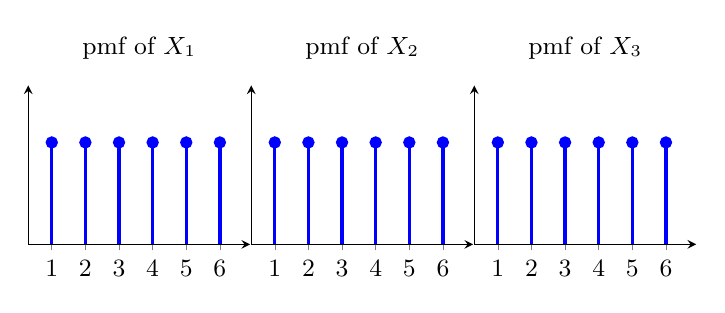
\begin{tikzpicture}
	\begin{axis}[name=p1, axis lines=left, xmin=0.3, xmax=6.9, ymin=0, ymax=0.26, xtick={1,...,6}, ytick=\empty, tick label style={font=\small}, title={pmf of $X_1$}, title style={font=\small}, width=4.4cm, height=3.6cm, clip=false]
		\addplot[ycomb, blue, very thick, mark=*, mark size=1.6pt] coordinates {(1,0.1667) (2,0.1667) (3,0.1667) (4,0.1667) (5,0.1667) (6,0.1667)};
	\end{axis}
	\begin{axis}[name=p2, at={(p1.outer east)}, anchor=outer west, axis lines=left, xmin=0.3, xmax=6.9, ymin=0, ymax=0.26, xtick={1,...,6}, ytick=\empty, tick label style={font=\small}, title={pmf of $X_2$}, title style={font=\small}, width=4.4cm, height=3.6cm, clip=false]
		\addplot[ycomb, blue, very thick, mark=*, mark size=1.6pt] coordinates {(1,0.1667) (2,0.1667) (3,0.1667) (4,0.1667) (5,0.1667) (6,0.1667)};
	\end{axis}
	\begin{axis}[name=p3, at={(p2.outer east)}, anchor=outer west, axis lines=left, xmin=0.3, xmax=6.9, ymin=0, ymax=0.26, xtick={1,...,6}, ytick=\empty, tick label style={font=\small}, title={pmf of $X_3$}, title style={font=\small}, width=4.4cm, height=3.6cm, clip=false]
		\addplot[ycomb, blue, very thick, mark=*, mark size=1.6pt] coordinates {(1,0.1667) (2,0.1667) (3,0.1667) (4,0.1667) (5,0.1667) (6,0.1667)};
	\end{axis}
	
\end{tikzpicture}
\end{document}
